% Options for packages loaded elsewhere
\PassOptionsToPackage{unicode}{hyperref}
\PassOptionsToPackage{hyphens}{url}
\PassOptionsToPackage{dvipsnames,svgnames,x11names}{xcolor}
%
\documentclass[
  letterpaper,
  DIV=11,
  numbers=noendperiod]{scrreprt}

\usepackage{amsmath,amssymb}
\usepackage{iftex}
\ifPDFTeX
  \usepackage[T1]{fontenc}
  \usepackage[utf8]{inputenc}
  \usepackage{textcomp} % provide euro and other symbols
\else % if luatex or xetex
  \usepackage{unicode-math}
  \defaultfontfeatures{Scale=MatchLowercase}
  \defaultfontfeatures[\rmfamily]{Ligatures=TeX,Scale=1}
\fi
\usepackage{lmodern}
\ifPDFTeX\else  
    % xetex/luatex font selection
\fi
% Use upquote if available, for straight quotes in verbatim environments
\IfFileExists{upquote.sty}{\usepackage{upquote}}{}
\IfFileExists{microtype.sty}{% use microtype if available
  \usepackage[]{microtype}
  \UseMicrotypeSet[protrusion]{basicmath} % disable protrusion for tt fonts
}{}
\makeatletter
\@ifundefined{KOMAClassName}{% if non-KOMA class
  \IfFileExists{parskip.sty}{%
    \usepackage{parskip}
  }{% else
    \setlength{\parindent}{0pt}
    \setlength{\parskip}{6pt plus 2pt minus 1pt}}
}{% if KOMA class
  \KOMAoptions{parskip=half}}
\makeatother
\usepackage{xcolor}
\setlength{\emergencystretch}{3em} % prevent overfull lines
\setcounter{secnumdepth}{5}
% Make \paragraph and \subparagraph free-standing
\makeatletter
\ifx\paragraph\undefined\else
  \let\oldparagraph\paragraph
  \renewcommand{\paragraph}{
    \@ifstar
      \xxxParagraphStar
      \xxxParagraphNoStar
  }
  \newcommand{\xxxParagraphStar}[1]{\oldparagraph*{#1}\mbox{}}
  \newcommand{\xxxParagraphNoStar}[1]{\oldparagraph{#1}\mbox{}}
\fi
\ifx\subparagraph\undefined\else
  \let\oldsubparagraph\subparagraph
  \renewcommand{\subparagraph}{
    \@ifstar
      \xxxSubParagraphStar
      \xxxSubParagraphNoStar
  }
  \newcommand{\xxxSubParagraphStar}[1]{\oldsubparagraph*{#1}\mbox{}}
  \newcommand{\xxxSubParagraphNoStar}[1]{\oldsubparagraph{#1}\mbox{}}
\fi
\makeatother


\providecommand{\tightlist}{%
  \setlength{\itemsep}{0pt}\setlength{\parskip}{0pt}}\usepackage{longtable,booktabs,array}
\usepackage{calc} % for calculating minipage widths
% Correct order of tables after \paragraph or \subparagraph
\usepackage{etoolbox}
\makeatletter
\patchcmd\longtable{\par}{\if@noskipsec\mbox{}\fi\par}{}{}
\makeatother
% Allow footnotes in longtable head/foot
\IfFileExists{footnotehyper.sty}{\usepackage{footnotehyper}}{\usepackage{footnote}}
\makesavenoteenv{longtable}
\usepackage{graphicx}
\makeatletter
\def\maxwidth{\ifdim\Gin@nat@width>\linewidth\linewidth\else\Gin@nat@width\fi}
\def\maxheight{\ifdim\Gin@nat@height>\textheight\textheight\else\Gin@nat@height\fi}
\makeatother
% Scale images if necessary, so that they will not overflow the page
% margins by default, and it is still possible to overwrite the defaults
% using explicit options in \includegraphics[width, height, ...]{}
\setkeys{Gin}{width=\maxwidth,height=\maxheight,keepaspectratio}
% Set default figure placement to htbp
\makeatletter
\def\fps@figure{htbp}
\makeatother
% definitions for citeproc citations
\NewDocumentCommand\citeproctext{}{}
\NewDocumentCommand\citeproc{mm}{%
  \begingroup\def\citeproctext{#2}\cite{#1}\endgroup}
\makeatletter
 % allow citations to break across lines
 \let\@cite@ofmt\@firstofone
 % avoid brackets around text for \cite:
 \def\@biblabel#1{}
 \def\@cite#1#2{{#1\if@tempswa , #2\fi}}
\makeatother
\newlength{\cslhangindent}
\setlength{\cslhangindent}{1.5em}
\newlength{\csllabelwidth}
\setlength{\csllabelwidth}{3em}
\newenvironment{CSLReferences}[2] % #1 hanging-indent, #2 entry-spacing
 {\begin{list}{}{%
  \setlength{\itemindent}{0pt}
  \setlength{\leftmargin}{0pt}
  \setlength{\parsep}{0pt}
  % turn on hanging indent if param 1 is 1
  \ifodd #1
   \setlength{\leftmargin}{\cslhangindent}
   \setlength{\itemindent}{-1\cslhangindent}
  \fi
  % set entry spacing
  \setlength{\itemsep}{#2\baselineskip}}}
 {\end{list}}
\usepackage{calc}
\newcommand{\CSLBlock}[1]{\hfill\break\parbox[t]{\linewidth}{\strut\ignorespaces#1\strut}}
\newcommand{\CSLLeftMargin}[1]{\parbox[t]{\csllabelwidth}{\strut#1\strut}}
\newcommand{\CSLRightInline}[1]{\parbox[t]{\linewidth - \csllabelwidth}{\strut#1\strut}}
\newcommand{\CSLIndent}[1]{\hspace{\cslhangindent}#1}

\KOMAoption{captions}{tableheading}
\makeatletter
\@ifpackageloaded{bookmark}{}{\usepackage{bookmark}}
\makeatother
\makeatletter
\@ifpackageloaded{caption}{}{\usepackage{caption}}
\AtBeginDocument{%
\ifdefined\contentsname
  \renewcommand*\contentsname{Table of contents}
\else
  \newcommand\contentsname{Table of contents}
\fi
\ifdefined\listfigurename
  \renewcommand*\listfigurename{List of Figures}
\else
  \newcommand\listfigurename{List of Figures}
\fi
\ifdefined\listtablename
  \renewcommand*\listtablename{List of Tables}
\else
  \newcommand\listtablename{List of Tables}
\fi
\ifdefined\figurename
  \renewcommand*\figurename{Figure}
\else
  \newcommand\figurename{Figure}
\fi
\ifdefined\tablename
  \renewcommand*\tablename{Table}
\else
  \newcommand\tablename{Table}
\fi
}
\@ifpackageloaded{float}{}{\usepackage{float}}
\floatstyle{ruled}
\@ifundefined{c@chapter}{\newfloat{codelisting}{h}{lop}}{\newfloat{codelisting}{h}{lop}[chapter]}
\floatname{codelisting}{Listing}
\newcommand*\listoflistings{\listof{codelisting}{List of Listings}}
\makeatother
\makeatletter
\makeatother
\makeatletter
\@ifpackageloaded{caption}{}{\usepackage{caption}}
\@ifpackageloaded{subcaption}{}{\usepackage{subcaption}}
\makeatother

\ifLuaTeX
  \usepackage{selnolig}  % disable illegal ligatures
\fi
\usepackage{bookmark}

\IfFileExists{xurl.sty}{\usepackage{xurl}}{} % add URL line breaks if available
\urlstyle{same} % disable monospaced font for URLs
\hypersetup{
  pdftitle={Getting Started with R for Economists},
  pdfauthor={Priyanga Dilini Talagala},
  colorlinks=true,
  linkcolor={blue},
  filecolor={Maroon},
  citecolor={Blue},
  urlcolor={Blue},
  pdfcreator={LaTeX via pandoc}}


\title{Getting Started with R for Economists}
\author{Priyanga Dilini Talagala}
\date{2025-01-06}

\begin{document}
\maketitle

\renewcommand*\contentsname{Table of contents}
{
\hypersetup{linkcolor=}
\setcounter{tocdepth}{2}
\tableofcontents
}

\bookmarksetup{startatroot}

\chapter*{Preface}\label{preface}
\addcontentsline{toc}{chapter}{Preface}

\markboth{Preface}{Preface}

R is a free and powerful software environment for statistical computing
and data visualization. It is widely used in academia and industry for
data analysis and research. As one of the top programming languages for
data science, R provides a variety of tools for statistical modeling,
computing, and visualization.

Since empirical research is essential in economics, programming skills
are crucial for conducting real-world data analysis. This textbook will
introduce you to R and help you develop fundamental data science skills.

\subsection*{\texorpdfstring{\textbf{About This
Book}}{About This Book}}\label{about-this-book}
\addcontentsline{toc}{subsection}{\textbf{About This Book}}

This textbook is designed for beginners, providing a strong foundation
in R for economic research. It focuses on \textbf{the tidyverse}
ecosystem, a collection of R packages that provide a simple yet powerful
approach to data analysis. You will learn how to use tidy tools to
manage and analyze data efficiently, covering the entire lifecycle of a
data science project.

\bookmarksetup{startatroot}

\chapter{Introduction to R and
RStudio}\label{introduction-to-r-and-rstudio}

\section{Installing R and Rstudio}\label{installing-r-and-rstudio}

\begin{itemize}
\item
  \textbf{Step 1:} First download R freely from the Comprehensive R
  Archive Network (CRAN) \url{https://cran.r-project.org/}. (At the
  moment of writing, R 4.4.2 is the latest version. Choose the most
  recent one.)
\item
  \textbf{Step 2:} Then install R Studio's IDE (stands for integrated
  development environment), a powerful user interface for R from
  {[}https://posit.co/download/rstudio-desktop/{]}(https://posit.co/download/rstudio-desktop/.
  Get the Open Source Edition of RStudio Desktop. RStudio allows you to
  run R in a more user-friendly environment.

  \begin{itemize}
  \item
    You need to install \textbf{both} R and Rstudio to use RStudio.
  \item
    If you have a pre-existing installation of R and/or RStudio, I
    highly recommend that you reinstall both and get as current as
    possible.
  \end{itemize}
\item
  \textbf{Step 3:} Then open \textbf{Rstudio}.
\end{itemize}

\subsection{Posit Cloud}\label{posit-cloud}

\begin{itemize}
\item
  In 2022, RStudio changed its corporate name to Posit with the aim of
  expanding its focus beyond R to include users of Python and Visual
  Studio Code.
\item
  If you don't want to download or install R and R Studio, you can use
  RStudio on \hyperref[posit-cloud]{Posit Cloud} (https://posit.cloud/)
  for free.
\end{itemize}

\section{RStudio layout}\label{rstudio-layout}

The RStudio interface consists of four panes: See Figure 1)

\begin{enumerate}
\def\labelenumi{\arabic{enumi}.}
\item
  \textbf{Source pane}
\item
  \textbf{Console pane}: This is where you type and run all your R
  commands.
\item
  \textbf{Environment pane}, containing the Environment, History,
  Connections, Build, and Tutorial tabs
\item
  \textbf{Output pane}, containing the Files, Plots, Packages, Help,
  Viewer, and Presentation tabs
\end{enumerate}

\begin{center}
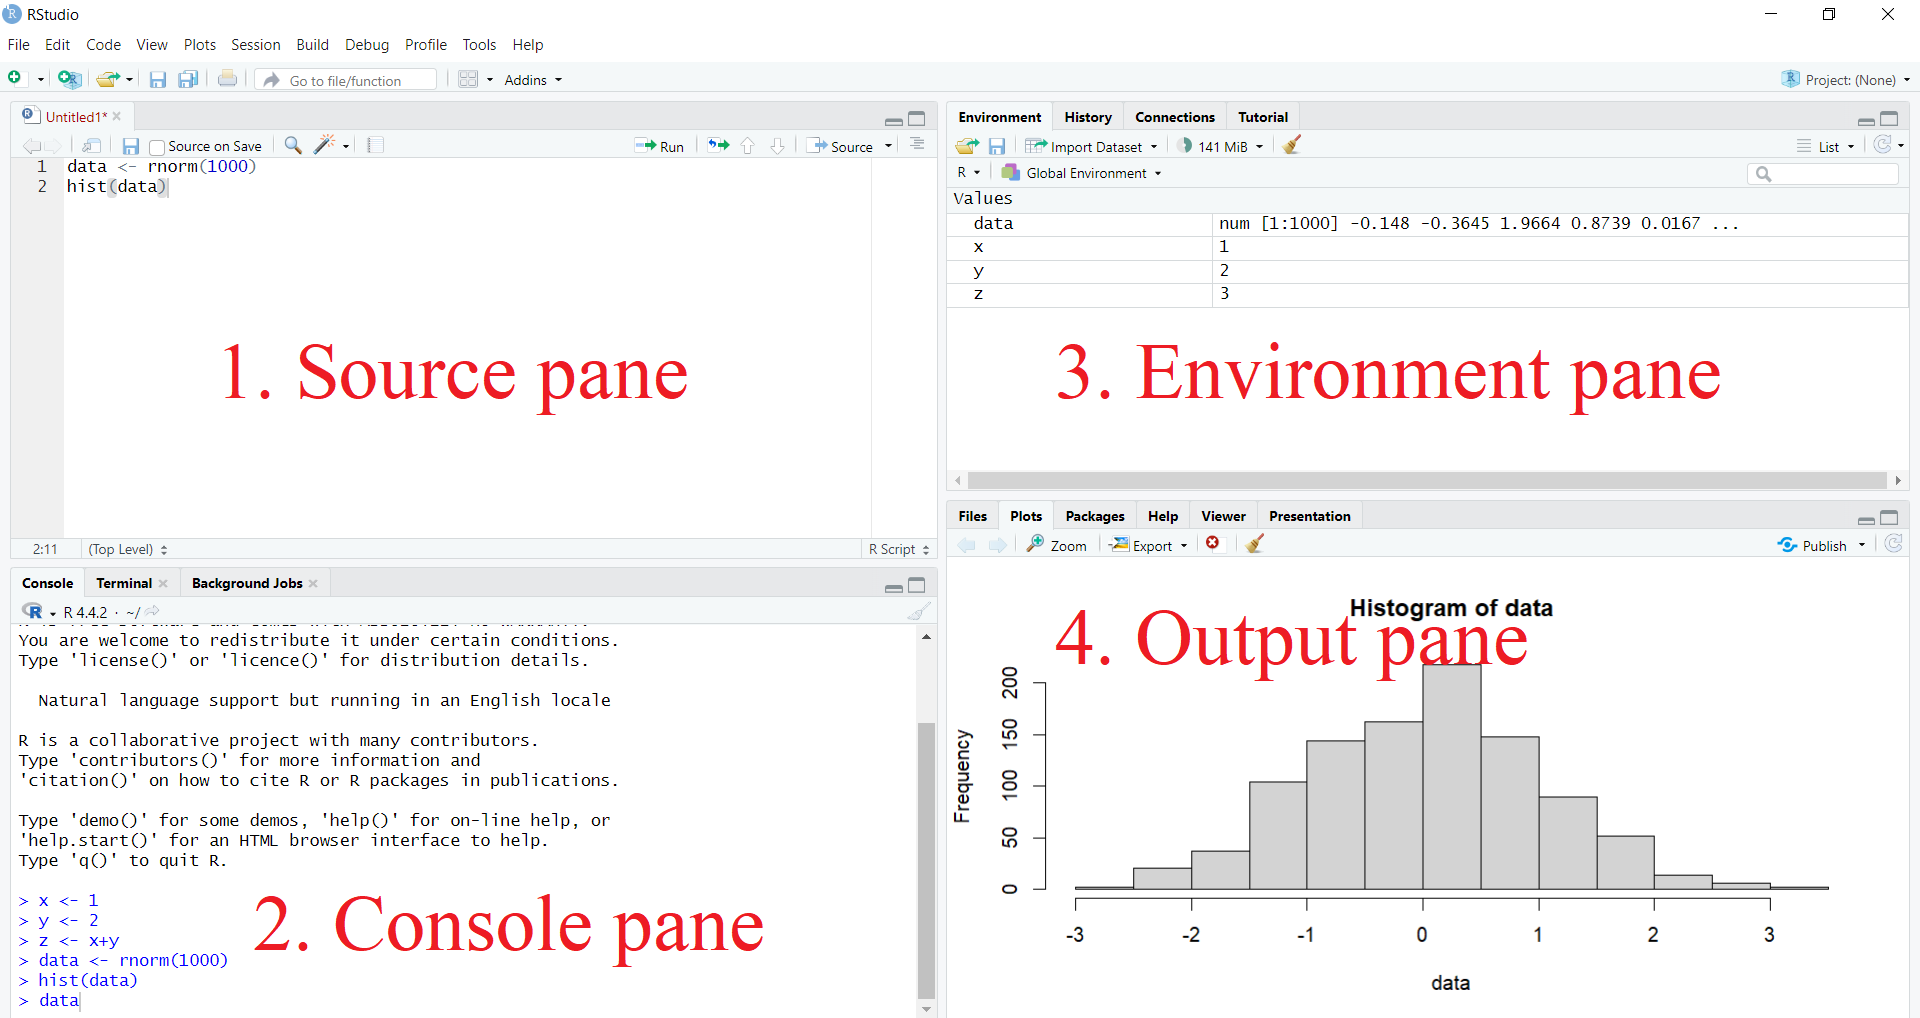
\includegraphics[width=1\textwidth,height=\textheight]{fig/1_Rstudio_Layout.png}
\end{center}

\bookmarksetup{startatroot}

\chapter{R Programming Basics}\label{r-programming-basics}

\bookmarksetup{startatroot}

\chapter{Reproducible Reporting with
Quarto}\label{reproducible-reporting-with-quarto}

\bookmarksetup{startatroot}

\chapter{Data Import and Export}\label{data-import-and-export}

\bookmarksetup{startatroot}

\chapter{Reproducible Reporting with
Quarto}\label{reproducible-reporting-with-quarto-1}

\bookmarksetup{startatroot}

\chapter{Data Wrangling}\label{data-wrangling}

\bookmarksetup{startatroot}

\chapter{Data Visualization}\label{data-visualization}

\bookmarksetup{startatroot}

\chapter{Introduction to Statistical
Modelling}\label{introduction-to-statistical-modelling}

\bookmarksetup{startatroot}

\chapter*{References}\label{references}
\addcontentsline{toc}{chapter}{References}

\markboth{References}{References}

\phantomsection\label{refs}
\begin{CSLReferences}{0}{1}
\end{CSLReferences}




\end{document}
